% !TeX spellcheck = da_DK
\subsection{Feedback}
\subsubsection{Teori og design} \label{Afs_Komparator}
Jævnfør afsnit \ref{Komparatorafsnit}, side \pageref{Komparatorafsnit} anvendes en komparator til at sammenligne to inputsspændinger. Der anvendes en komparator af typen LM$311$, hvis pinkonfiguration ses på \figref{fig:LM311}. LM$311$ har et arbejdsområde på $\pm15$V og skal forsynes med minimum $\pm3.5$V. 
\begin{figure}[H] 
	\centering
	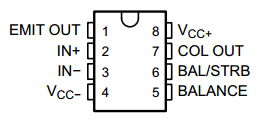
\includegraphics[scale=0.9]{figures/cProblemloesning/LM311.PNG}
	\caption{På figuren ses pinkonfigurationen for komparatoren LM$311$ \cite{Instruments2015}.}
	\label{fig:LM311}
\end{figure}
\noindent LM$311$ har to inputterminaler, hvilket ses som pin $2$ og $3$ på \figref{fig:LM311}, hvilket gør det muligt at sammenligne en referencespænding med et inputsignal. Deruover har den to outputs grundet den indbyggede transistor; et emitteroutput og et collectoroutput, hvilket ses som pin $1$ og $7$ på \figref{fig:LM311}. Emitterouputtet benyttes i dette tilfælde oftest som ground, hvorimod collectoroutputtet oftest benyttes som den aktiverende outputterminal. Komparatorens balanceterminaler på pin $5$ og $6$ benyttes til modkoblinger, som f.eks. en hysterese-modkobling. Hvis der ikke benyttes en modkobling, placeres en $100$nF kondensator i en sammenkobling af komparatorens balanceterminaler for at gøre komparatoren mere præcis og undgå svingninger \cite{Instruments2015}. 
Der anvendes flere komparatorer i feedbackblokken, hvor outputterminalen tilkobles et feedbackkomponent, samt en modstand og den positive spændingsforsyning ($V_{cc}$). Til vibratoren kobles yderligere den positive spændingsforsyning ($V_+$) på $3.4$V. Afhængig af det ønskede output kobles referencespændingen til den inverterende eller ikke-inverterende terminal på komparatoren. Hvis referencespændingen er tilkoblet den inverterende terminal, skal inputsignalet være mindre end denne for at aktivere feedbackkomponentet, der er placeret i komparatorens collectoroutput. Hvis referencespændingen er tilkoblet den ikke-inverterende terminal, skal inputsignalet være større end denne for at aktivere feedbackkomponentet. Komparatorerne kan derfor have to forskellige outputs afhængig af inputspændingen, som der ses på \figref{fig:komparator_forstaeelse}. 
\begin{figure}[H] 
	\centering
	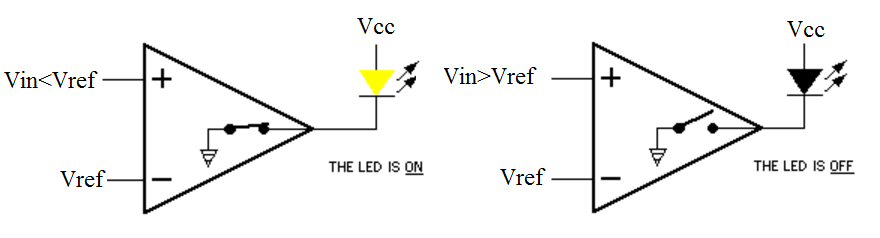
\includegraphics[scale=0.9]{figures/cProblemloesning/komparator_forstaeelse.PNG}
	\caption{På figuren ses en komparatorkonfiguration, hvor LED'en aktiveres efter forholdet mellem $V_{in}$ og $V_{ref}$. Der ses, at referencespændingen er tilkoblet den inverterende terminal, hvorfor LED'en aktiveres, når $V_{in}$ er mindre end $V_{ref}$. LED'en er derimod inaktiv, når $V_{in}$ er større end $V_{ref}$. (Revideret) \cite{Paisley2015}.}
	\label{fig:komparator_forstaeelse}
\end{figure}
\noindent På \figref{fig:komparator_forstaeelse} kan det ses at aktivering af LED'en afhænger af, om strømmen kan løbe til ground. Hvis dette ikke er muligt, kan der ikke ske et spændingsfald over LED'en, hvorfor den ikke aktiveres. %Hvis strømmen ikke kan dette vil det også være umuligt for strømmen at løbe igennem LED'en, og der vil derved heller ikke ske et spændingsfald over LED'en. 
%Hvis inputsignalet ligger under de beregnede tærskelværdier vil outputtet være $0$V og LEDerne samt de to vibratorer vil ikke blive aktiveret. 
%Er inputtet derimod over de beregnede tærskelværdier, vil outputtet svare til ground, da strømmen fra $+V_{cc}$ vil løbe igennem komparatorerne og derefter til ground\fxnote{det vil vel løbe til komparatorens emitter terminal }. Derved opnås et spændingsfald over den positive pol \fxnote{anode} og den negative pol \fxnote{katode} for LEDerne og vibratorerne på en værdi, der ligger over det minimale spændingsfald, der kræves for en aktivering. LEDerne og vibratorerne vil derved blive aktiveret og fungere som feedback til patienten. \\

\noindent Komparatoren LM$311$ har en lav indgangsimpedans, hvorfor der placeres en buffer mellem outputtet fra tilpasningsblokken og feedbackblokken, hvilket forhindrer loading, jævnfør afsnit \ref{Bilag:Pilotforsoeg}, side \pageref{Bilag:Pilotforsoeg} \cite{Instruments2015}. Jævnfør afsnit \ref{KomparatorAfs}, side \pageref{KomparatorAfs} skal LED'erne og vibratorerne aktiveres i fem forskellige stadier vha. hver sin komparator. Der anvendes i alt otte komparatorer. Den grønne LED's stadie har en positiv og negativ tærskelværdi, hvorfor denne kræver to komparatorer i en vindueskonfiguration. De valgte tærskelværdier kan designes som f.eks. to spændingstræer eller otte spændingsdelere, hvoraf der er fordele og ulemper ved begge metoder. Et eksempel på et spændingstræ og en spændingsdeler kan ses på \figref{fig:spaendingstrae}. 
\begin{figure}[H] 
	\centering
	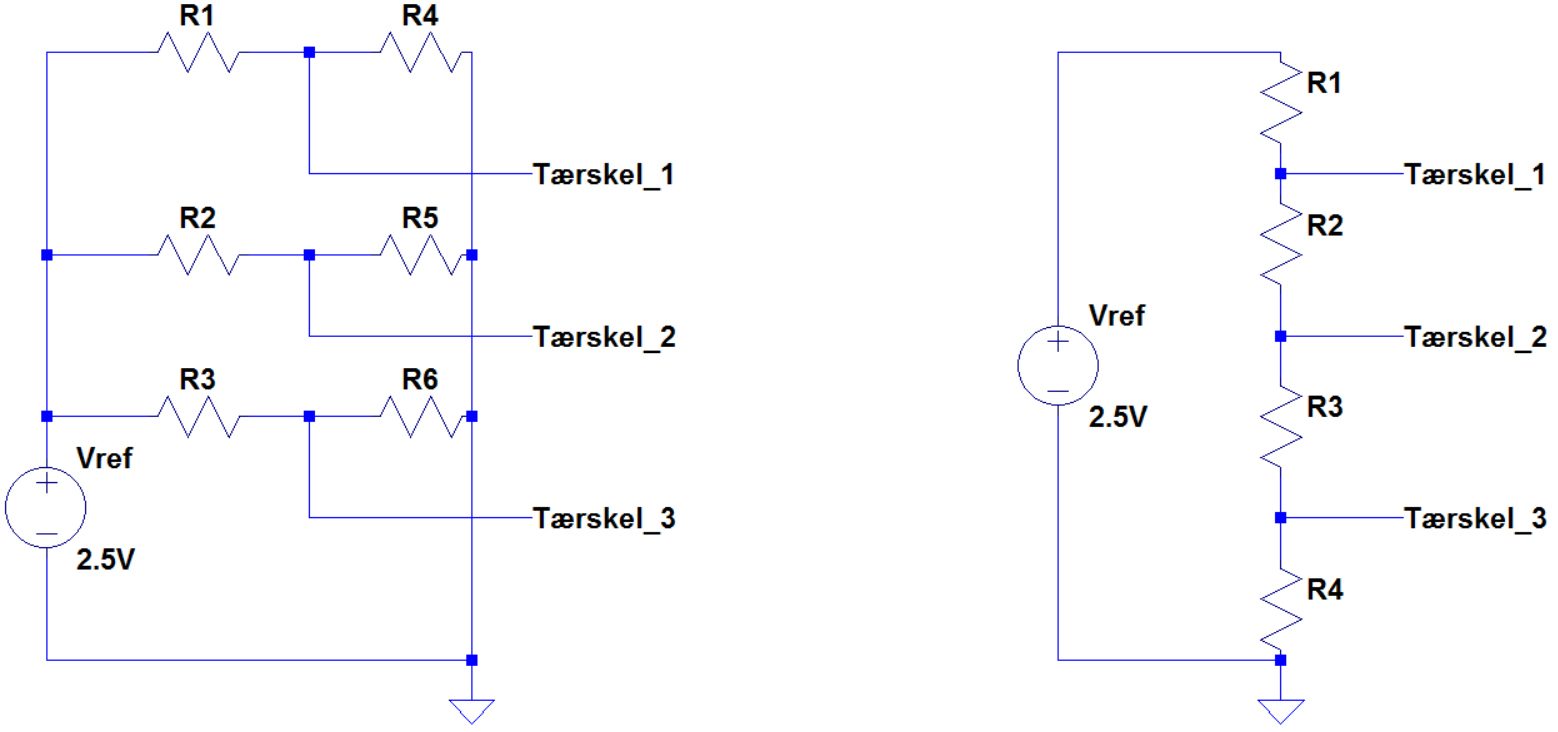
\includegraphics[scale=0.4]{figures/cProblemloesning/eksempel_speadingstrae.PNG}
	\caption{På figuren ses et eksempel på hhv. en individuel spændingsdelere og et spændingstræ.}
	\label{fig:spaendingstrae}
\end{figure}
\noindent Ud af de otte komparatorer anvendes seks af dem i en ordinær komparatorkonfiguration, som aktiveres ved en bestemt tærskelværdi vha. individuelle spændingsdelere. Fordelen ved at vælge dette design er, at modstandene ikke kan påvirke hinanden, hvilket de kan i et spændingstræ. Ulempen ved at anvende spændingsdelere er, at der benyttes flere modstande ved denne konfiguration, som kan afvige fra deres teoretiske værdier.\\
Feedbackblokken kan adskilles i to dele ved den grønne LED; en for hældning i hhv. positiv og negativ retning. Der indgår $12$ modstande (R$1$-R$12$) i de fem spændingsdelere, som leverer tærskelværdier til de otte komparatorer. Derudover består kredsløbet af en spændingsreference ($+V_{ref}$) på $2.5$V, jævnfør afsnit \ref{subsec:Spaendingsref_Komparator}, side \pageref{subsec:Spaendingsref_Komparator}, og syv modstande (R$13$-R$19$) mellem LED'erne samt vibratorerne og $V_{cc}$. Modstandene (R$13$-R$14$, R$16$-R$17$ og R$19$) bestemmer strømforsyningen til LED'erne\fxnote{NTK: R$15$ og R$18$ er placeret ved spændingsforsyningen på $5.5$V ($V_{cc}$) og bestemmes til at være $100$K$\Omega$. Disse skal sørge for at kredsløbet ikke bruger for meget strøm, hvorfor der er valgt modstande med en høj værdi.}. Vindueskonfigurationen designes ved at placere en LED (D$3$) i emitterterminalen på komparatoren (U$3$) og collectorterminalen på komparatoren (U$4$). Feedbackblokken fremgår af \figref{fig:komparator_uden_vaerdi}. 

\begin{figure}[H] 
	\centering
	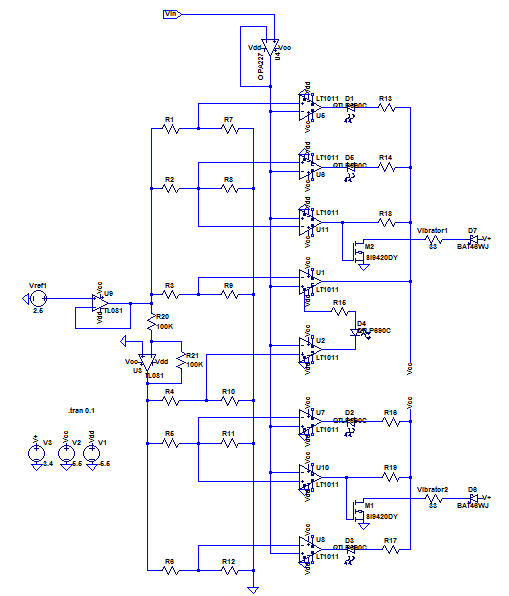
\includegraphics[scale=0.4]{figures/cProblemloesning/komparator_uden_vaerdi.PNG}
	\caption{På figuren ses feedbackblokken, som kan adskilles i to dele ved den grønne LED; en for hældning i hhv. positiv og negativ retning. Der indgår $12$ modstande (R$1$-R$12$) i de fem spændingsdelere, som leverer tærskelværdier til de otte komparatorer. Derudover indgår en spændingsreference på $2.5$V. Der ses yderligere dem LED'er og to vibratorer, hvilket fremgår som to modstande i LTspice, samt tilhørende modstande. For den grønne LED er der en vindueskonfigurationen konstrueret vha. komparatorerne (U$3$-U$4$).}
	\label{fig:komparator_uden_vaerdi}
\end{figure}

%%%%%%%%%%%%%%%%%%%%%%%%%%%%%%%%%%%%%%%%%%%%%%%%%%%%%%%%%%%%%%%

\noindent\textbf{Beregning af tærskelværdier og modstandene R$1$-R$12$ i spændingsdelerne} \\
Der kræves at LED'erne skal lyse ved bestemte tærskelværdier, dvs. bestemte kropshældninger, jævnfør afsnit \ref{KomparatorAfs}, side \pageref{KomparatorAfs}. Inputsignalet afhænger af den pågældende hældningsgrad, da denne bestemmer inputspændingen til komparatorerne. Tærskelværdier kan beregnes, da værdien i volt pr. grad i hhv. positiv og negativ retning er kendt, jævnfør \eqref{taeskelvaerdi_pr_grad}, side \pageref{Sec_Pilot_Data}. Desuden kendes forstærkningsfaktoren fra de tidligere blokke. Tærskelværdierne for komparatoren beregnes ud fra følgende formler:
\begin{eqnarray} \label{pr_grad} 
Positiv-retning : 0.0037\text{V} \cdot 9.1 \cdot 3.6 \cdot \text{hældning} = \text{tærskelværdi} \\
Negativ-retning : 0.0036\text{V} \cdot 9.1 \cdot 3.6 \cdot \text{hældning} = \text{tærskelværdi}
\end{eqnarray}
\noindent Hvor $0.0037$ og $0.0036$ er volten pr. grad i hhv. positiv og negativ retning. Værdierne $9.14$ og $3.6$ er forstærkningsfaktoren fra de forrige blokke, og hældningen er den grad, som tærskelværdien skal indstilles efter. 
De udregnede tærskelværdier fremgår af \figref{fig:taerskelvaerdier}. 
\begin{figure}[H]
	\centering
	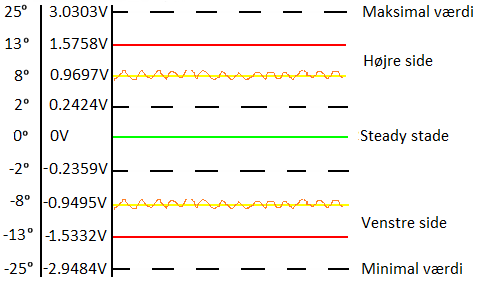
\includegraphics[scale=1.]{figures/cProblemloesning/Taerskelvaerdier.PNG}
	\caption{Af figuren fremgår de beregnede tærskelværdier. Farverne angiver hvilket LED, der skal aktiveres ved de enkelte tærskelværdier. Derudover angiver de orange linjer aktiveringen af vibratorerne. Arbejdsområdet angives som den maksimale og minimale værdi.}
	\label{fig:taerskelvaerdier}
\end{figure}

\noindent Der anvendes en spændingsreference, som kan levere en konstant spænding på $2.5$V til feedbackkonfigurationen jævnfør afsnit \ref{subsec:Spaendingsref_Komparator}, side \pageref{subsec:Spaendingsref_Komparator}. Denne benyttes, da spændingen fra et batteri vil falde over tid. 
Da spændingsreferencen yderligere skal anvendes til at definere de negative tærskelværdier benyttes en inverterende forstærker med et gain på $1$, hvilket fremgår af \figref{fig:komparator_uden_vaerdi}. Ved denne konfiguration inverteres signalet uden at blive forstærket. \\
For at bestemme R$1$-R$12$ i spændingsdelerne fastsættes R$1$-R$6$ til en bestemt værdi på $10$K$\Omega$. Tærskelværdierne ($V_{out}$) og spændingsreferencen ($V_{in}$) er kendte værdier, hvormed R$7$-R$12$ kan udregnes vha. den generelle formel for en spændingsdeler, jævnfør \eqref{eq:Spaendingsdeler}, side \pageref{subsec:Spaendingsref}. De beregnede værdier for R$7$-R$12$ ses i \tableref{tab:modtande_R7-R12}.
\begin{table}[H]
	\centering
	\begin{tabular}{|l|l|l|l|} \hline
		\textit{Modstand} & \textit{Værdi}
	\textit{R$7$} & $16.821$K$\Omega$ \\ \hline
	\textit{R$8$} & $6.285$K$\Omega$ \\ \hline
	\textit{R$9$} & $1.068$K$\Omega$ \\ \hline
	\textit{R$10$} & $1.042$K$\Omega$ \\ \hline
	\textit{R$11$} & $6.039$K$\Omega$ \\ \hline
	\textit{R$12$} & $15.765$K$\Omega$ \\ \hline    
	\end{tabular}
	\caption{I tabellen ses de beregnede værdier for R$7$-R$12$.}
	\label{tab:modtande_R7-R12}
\end{table}

%%%%%%%%%%%%%%%%%%%%%%%%%%%%%%%%%%%%%%%%%%%%%%%%%%%%%%%%

\noindent\textbf{Beregning af modstande for den visuelle del af feedbacken} \\
Til den visuelle del af feedbacken anvendes LED'er. En LED har to terminaler; en anode og en katode, hvoraf katoden tilkobles komparatorens output mens anoden tilkobles $V_{cc}$. En ideel LED tændes, når der løber strøm fra anoden til katoden, hvorved der opstår et spændingsfald over LED'en. Dette kaldes fremadgående spænding. I praksis vil der altid løbe en lækstrøm i LED'en, hvilket vil give et spændingsfald. Når strømmen løber fra katoden til anoden, vil LED'en være slukket, da der ideelt ikke løber strøm igennem kredsløbet. \cite{Sedra2010} \\
Jænvfør afsnit \ref{KomparatorAfs}, side \pageref{KomparatorAfs} skal spændingensforsyningen være $5.5$V. De anvendte LED'er i systemet er: en grøn L-$53$LG $5$mm (D$3$), to gule L-$53$LY $5$mm (D$2$ og D$4$) og to røde L-$53$LI $5$mm (D$1$ og D$5$). LED'erne kræver en minimum strøm på $2$mA for at lyse og $20$mA, hvis de skal give et tydeligt lys. Hvis LED'erne forsynes med mere end $150$mA, brænder de af. Spændingsfaldet over LED'erne afhængder af den strøm der løber igennem dem. Ved $2$mA ligger det typisk mellem $1.7$V-$1.9$V\fxnote{NTK:rød: $1.7$, gul: $1.8$ og grøn: $1.9$}. 
Spændingsforsyningen tilkobles tilhørende modstande for at kontrollere strømmen til LED'erne. \cite{kingbright} Spændingsfaldet over LED'erne samt den strøm LED'erne skal bruge for at lyse tydeligt, er kendte værdier, hvorfor modstandene R$13$-R$14$, R$16$-R$17$ og R$19$ kan findes vha. Ohms lov. Nedenstående udregning beregner værdien af modstandene, hvis spændingsforsyningen forsyner kredsløbet med $5.5$V og LED'erne med $20$mA:

%Til den visuelle del af feedbackkonfigurationen anvendes LEDer. En LED har to terminaler; en anode og en katode. Når en ideel LED tændes skyldes det, at der løber strøm fra anoden til katoden og der vil her være et spændingsfald over LEDen på 0V. Dette kaldes fremadgående spændings. Når strømmen løber fra katoden til anoden vil LEDen være slukket, da der ideelt ikke løber strøm igennem kredsløbet. \fxnote{tilføjes mere til teori af LED}
%Jænvfør kravspecifikationerne i afsnit \ref{KomparatorAfs} på side \pageref{KomparatorAfs} for komparatoren skal forsyningsspændingen være $5.5$V. De anvendte LEDer i systemet er: en grøn L-$53$LG $5$mm (D$3$), to gule L-$53$LY $$5$mm (D$2$ og D$4$) og to røde L-$53$LI $5$mm (D$1$ og D$5$). LEDerne kræver en minimum strøm på $2$mA for at lyse og $20$mA hvis de skal give et tydeligt lys.  Spændingsfaldet over LED-dioderne ligger maksimalt i intervallet $2.0$V til $2.2$ V (rød: $2.0$, gul: $2.1$ og grøn: $2.2$), men typisk mellem $1.7$V-$1.9$V. LED-dioderne skal derudover forsynes med $2$mA for at fungere, men kan forsynes op til \fxnote{Tjek og 150mA er rigtigt}$150$mA, før de brændes af. LEDerne forsynes af en $5.5$V spændingsforsyning og tilkobles, som sagt, tilhørende modstande for bla. at undgå at LED-dioderne brænder af. \cite{kingbright} Spændingsfaldet over dioderne samt den spænding LEDerne som minimum skal bruge for at lyse er kendte værdier, dvs. modstandene R$12$-R$17$ kan derfor findes vha. Ohms lov. Nedenstående udregning beregnet en værdi af modstandene, hvis spændingsforsyningen forsyner kredsløbet med $5.5$V og LEDernes med $20$mA for at aktiveres:

\begin{equation}
R$13$-R$14$, R$16$-R$17$\text{ og }R$19$ = \dfrac{5.5V - 2.2V}{0.02A} = 165\Omega
\end{equation}
\noindent Ud fra denne beregning sættes modstandene R$13$-R$14$, R$16$-R$17$ og R$19$ til $165\Omega$ for at sikre, at LED'erne forsynes med $20$mA. \\
Den visuelle del af feedbackkonfigurationen fremgår af \figref{fig:komparator_uden_vaerdi}

%%%%%%%%%%%%%%%%%%%%%%%%%%%%%%%%%%%%%%%%%%%%%%%%%%%%%%%%%%%


\noindent\textbf{Beregning af modstande for den somatosensoriske del af feedbacken} \\
Til den somatosensoriske del af feedbacken benyttes vibratorer, jævnfør afsnit \ref{KomparatorAfs}, side \pageref{KomparatorAfs}. En vibrator er en elektrisk motor, der skaber svingninger, hvilket medfører en vibration \cite{Redaktionen2009}. De anvendte vibratorer er af typen C$1026$B og har et driftsområde på $2.7$-$3.3$V, der typisk ligger på $3$V\fxnote{starter ved $2.3$V}. Vibratorerne skal derfor have en spændingsforsyning på mindst $2.7$V. Derudover er startstrømmen $120$mA, og driftsstrømmen er $90$mA. Herefter sker vibrationen med en frekvens på $10$-$55$Hz afhængig af spændingsforsyningen samt strømmen i kredsløbet. \cite{Machinery2009} %Jævnfør kravspecifikationerne benyttes vibratorerne med dimensionerne; $1$cm i diameter og $0.27$cm i tykkelse, så de kan påsættes patienternes hænder. 

For at opnå et tilstrækkeligt strømniveau anvendes en transistor af typen BS$170$. Transistoren placeres mellem komparatoren og vibratoren. Designet fungerer således, at transistoren tændes og vibratoren aktiveres, når komparatoren er slukket. Dette princip er modsat desginet af komparatorerne, som benyttes i forbindelse med aktivering af LED'erne. Dette skyldes, at når komparatoren er aktiveret, vil spændingen ledes til ground, som er tilkoblet komparatorens emitterterminal. Når komparatoren er slukket, vil spændingen aktivere transistorens gate-terminal. Modstandene R$15$ og R$18$ er placeret ved spændingsforsyningen på $5.5$V ($V_{cc}$) og bestemmes til at være $100$K$\Omega$. Disse skal sørge for, at kredsløbet ikke bruger for meget strøm. Når komparatoren slukker, vil spændingen aktivere transistoren og der dannes forbindelse mellem transistorens drain- og sourceterminal. Dette vil aktivere vibratorerne, da strømmen derved kan løbe til ground i sourceterminalen. Spændingsforsyningen til vibratorerne er på $3.4$V ($V+$) og forsynes af spændingsregulatoren. Eftersom vibratoren som nævnt skal forsynes med $2.7$V, anvendes en Schottky-diode af typen BAT$41$, der nedsætter spændingen til under $3$V. Schottky-dioden fungerer således, at der sker et spændingsfald, afhængig af strømmen, som løber igennem dioden. Spændingsforsyningen på $3.4$V forsyner, når komparatoren slukker og der er forbindelse mellem transistorens drain- og source-terminal, da strømmen kan løbe til ground i source-terminalen. Den somasensoriske del af feedbackkonfigurationen fremgår af \figref{fig:komparator_uden_vaerdi}.
 
\subsubsection{Simulering}\label{feedback_simulering}
Den visuelle og somatosensoriske del af feedbackblokken simuleres med et sinussignal som input, der har en amplitude på $3$V. Dette gøres for at simulere signalet fra den forrige blok, som har et arbejdsområde på $\pm3$V. I simuleringen testes der for, om feedbacken aktiveres ved de forskellige tærskelværdier, og tærskelværdierne i simuleringen måles.
%I simuleringen testes, hvorvidt tærskelværdierne kan accepteres ift. kravspecifikationer. 
%Kredsløbet simuleres ikke med en spændingsreference, men derimod en spændingsforsyning på $2.5$V, der indikerer spændingsreferencen. 
Af \figref{fig:komparator_samlet} fremgår feedbackblokken, der simuleres i LTspice.

\begin{figure}[H]
	\centering
	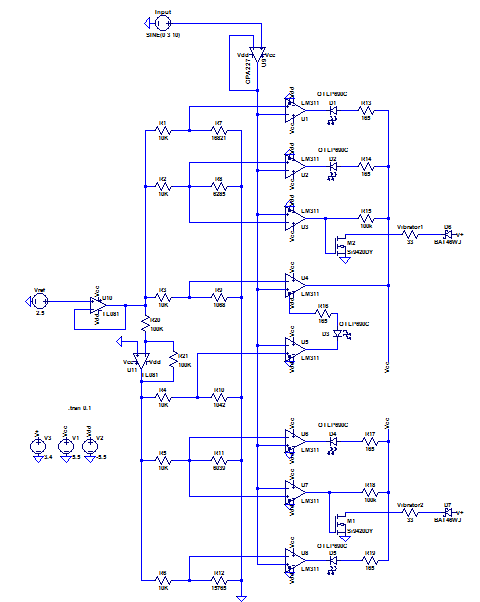
\includegraphics[scale=0.4]{figures/cProblemloesning/komparator_samlet.PNG}
	\caption{Af figuren fremgår feedbackkonfigurationen med beregnede modstande. Kredsløbet simuleres med et sinussignal som input, der har en amplitude på $3$V.}
	\label{fig:komparator_samlet}
\end{figure}
 
\noindent\textbf{Simulering af den visuelle del af feedbacken} \\
%Til simulering af den visuelle del af feedbackkonfiguration anvendes komparatorer af typen LM$311$ og LED'er af typen QTLP$690$C, da de reelle komponenter ikke kan vælges i LTspice.\fxnote{skal vi slette det med LM311?} Kredsløbet simuleres i LTspice for at teste, hvorvidt den visuelle del af feedbackkonfiguration opfylder de opstillede kravspecifikationer, jævnfør afsnit \ref{KomparatorAfs} på side \pageref{KomparatorAfs}.
Af \figref{fig:komparator_visuel_simulering_samlet1} fremgår tærskelværdierne for den visuelle del af feedbacken. 

\begin{figure}[H]
	\centering
	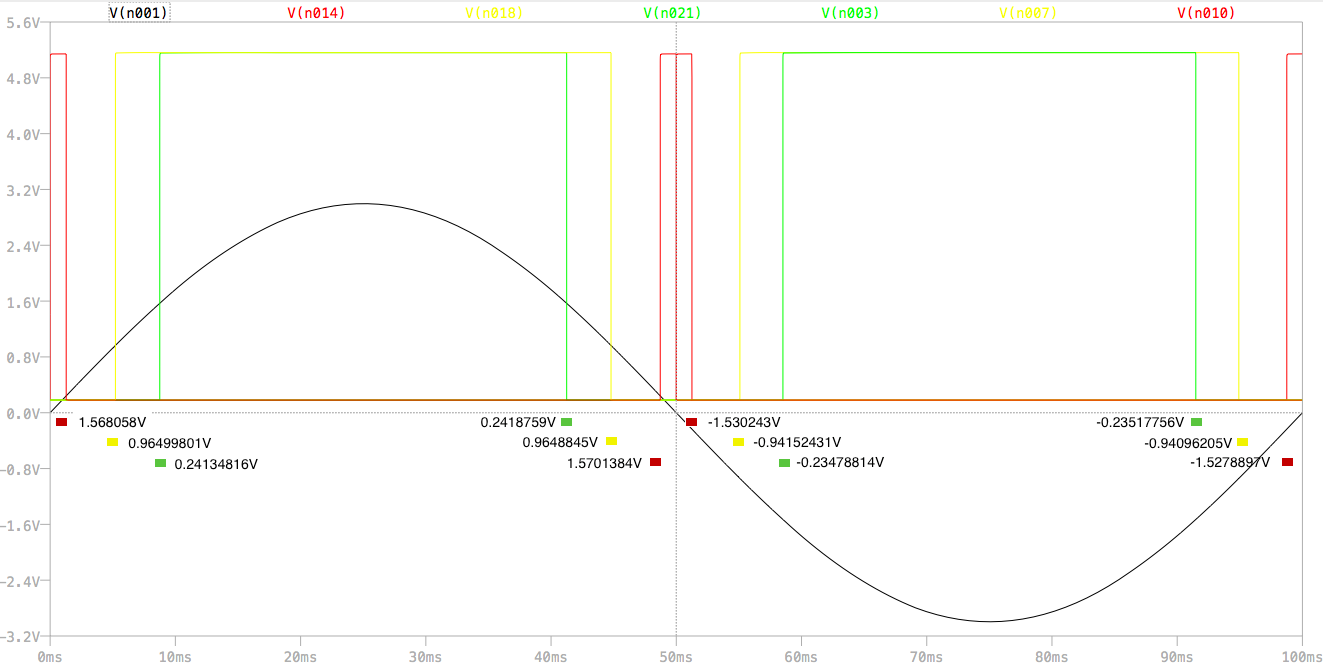
\includegraphics[scale=0.36]{figures/cProblemloesning/komparator_visuel_simulering_samlet1.PNG}
	\caption{På figuren ses simuleringen af den visuelle del af feedbacken. V(n$002$) er sinus-signalet, der illustrerer blokkens inputsignal. V(n$004$) viser spændingsfaldet for de røde LED'er, V(n$008$) for de gule LED'er og V(n$015$) for den grønne LED. Når inputsignalet når de definerede tærskelværdier, vil kurverne gå i negativ mætning og LED-dioderne vil lyse.}
	\label{fig:komparator_visuel_simulering_samlet1}
\end{figure}

\noindent På \figref{fig:komparator_visuel_simulering_samlet1} fremgår det, signalet går i negativ mætning ved de enkelte tærskelværdier, hvilket får LED'erne til at lyse. Afvigelsen mellem det teoretiske og simulerede referenceinput beregnes og vil fremgå af \tableref{Tab:test_reference1}.

\begin{table}[H]
	\centering
	\begin{tabular}{|l|l|l|l|} \hline
		& \textit{\begin{tabular}[c]{@{}l@{}}Teoretisk\\ reference\\ input\end{tabular}} & \textit{\begin{tabular}[c]{@{}l@{}}Simuleret\\ reference\\ input\end{tabular}} & \textit{Afvigelse} \\ \hline
		\textit{$13^{\circ}$}  & $1.5758$V                                                                      & $1.5659$V                                                                  & $0.63\%$              \\ \hline
		\textit{$8^{\circ}$}   & $0.9697$V                                                                      & $0.9654$V                                                                  & $0.44\%$              \\ \hline
		\textit{$2^{\circ}$}   & $0.2424$V                                                                      & $0.2415$V                                                                  & $0.37\%$              \\ \hline
		\textit{-$2^{\circ}$}  & -$0.2359$V                                                                     & -$0.2348$V                                                                 & $0.47\%$              \\ \hline
		\textit{-$8^{\circ}$}  & -$0.9495$V                                                                     & -$0.9341$V                                                                 & $0.92\%$              \\ \hline
		\textit{-$13^{\circ}$} & -$1.5332$V                                                                     & -$1.5320$V                                                                 & $0.08\%$        \\ \hline     
	\end{tabular}
	\caption{Af tabellen fremgår de teoretiske og simulerede tærskelværdier ved de enkelte hældningsgrader samt afvigelsen mellem disse.}
	\label{Tab:test_reference1}
\end{table}
\noindent Det kan udfra \tableref{Tab:test_reference1} konkluderes, at afvigelsen fra de udregnede tærskelværdier overholder tolerancerne, jævnfør afsnit \ref{KomparatorAfs}, side \pageref{KomparatorAfs}. På \figref{fig:vindues_konfiguration} ses en simulering af vindueskonfigurationen for den grønne LED. 
\begin{figure}[H]
	\centering
	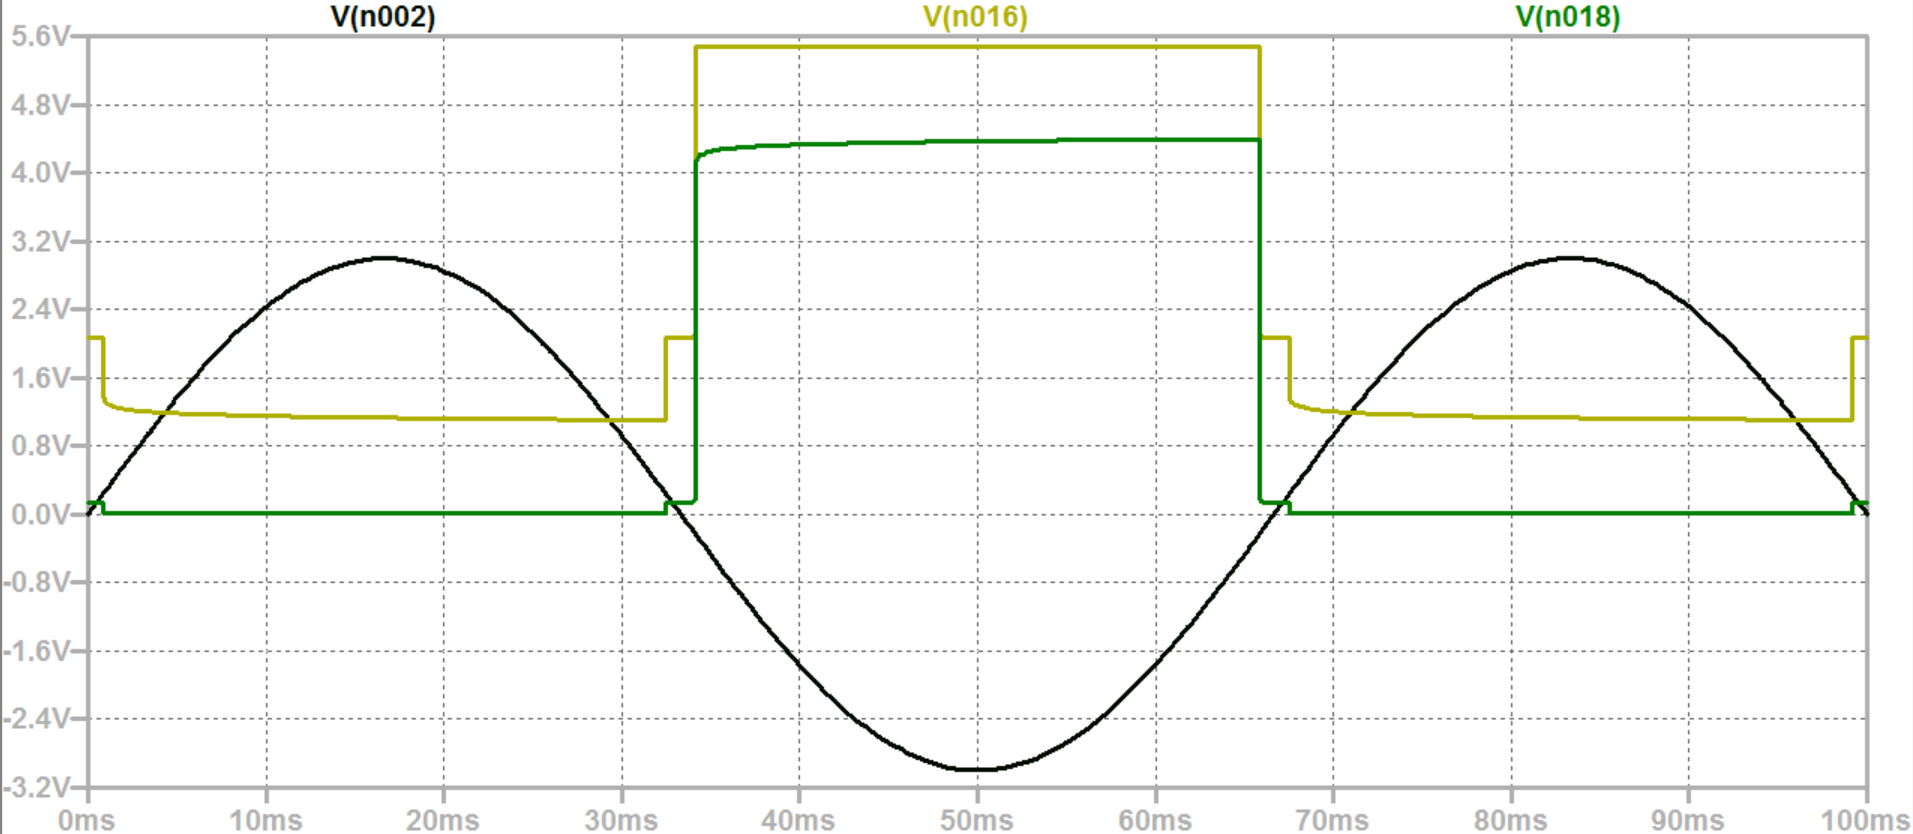
\includegraphics[scale=0.36]{figures/cProblemloesning/vindues_konfiguration.PNG}
	\caption{På figuren ses simuleringen af vindueskonfigurationen. V(n$002$) er sinus-signalet, der illustrerer blokkens inputsignal, V(n$016$) og V(n$018$) viser spændingsfaldet for den grønne LED.}
	\label{fig:vindues_konfiguration}
\end{figure}

%\begin{table}[H]
%	\centering
%	\begin{tabular}{|l|l|l|l|l|l|}
%		\hline
%					& \textit{Tærskelværdier} 	& \textit{Måling til højre} & \textit{Måling til venstre}		&  \textit{\begin{tabular}[c]{@{}l@{}}Afvigelse\\ for højre\end{tabular}}   &  \textit{\begin{tabular}[c]{@{}l@{}}Afvigelse\\ for venstre\end{tabular}}   \\ \hline
%\textbf{$2^{\circ}$} 		& $0.2412$V  				&$0.23815127$V 			&$-0.17571651$V		& $1.3\%$  &$??\%$ \\ \hline
% \textbf{$8^{\circ}$} 		&$0.9648$V					&$0.96551609$V			&$0.96777598$V		& $0.07\%$	&$0.3\%$\\ \hline
%\textbf{-$8^{\circ}$} 		&-$0.9413$V					&-$0.96784376$V 			&-$0.92251539$V		& $2.8\%$	&$2\%$\\ \hline 		
%\textbf{$13^{\circ}$} 		&$1.5679$V 					&$1.5583895$V 		  	&$1.5705552$V		& $0.6\%$	&$0.2\%$\\ \hline
%\textbf{-$13^{\circ}$} 		&-$1.5297$VV 				&-$1.5297296$V		   	&-$1.5297259$V		& $0.002\%$	&$0.002\%$ \\ \hline
%	\end{tabular}
%	\caption{I tabellen ses der, at de anvendte tærskelværdier afviger fra den teoretiske værdi, hvilket er forventet af reelle komponenter. Det er en acceptabel afvigelse, så tærskelværdierne kan derfor anvendes til implementering}
%	\label{Tab:Maalingtearskelvaerdier}
%\end{table}
\noindent Aktivering af vindueskonfigurationen sker ved, at den ene komparator vil åbne for spændingsforsyningen til LED'en. Herved kan $V_{cc}$ gå til LED'en gennem emitteroutputtet. Der vil ikke løbe strøm, hvilket ses ved, at den målte spænding ved LED'en er $5.5$V når U$4$ er tændt. Der vil være lys i LED'en, når U$5$ er tændt, da strømmen derved kan ledes til ground. Når U$4$ er slukket, vil der ikke være spændingsforsyning til LED'en uanset, om U$5$ er tændt eller slukket. \\
Den visuelle del af feedbacken overholder tolerancerne og kan derfor accepteres.\\ 

\noindent\textbf{Simulering af somatosensoriske del af feedbacken} \\
Til simuleringen af den somatosensoriske del af feedbacken anvendes modstande som vibratorer i LTspice. Deres værdi er beregnes vha. Ohms lov, hvilket fremgår af nedenstående \eqref{vibrator_modstand}:
\begin{equation} \label{vibrator_modstand}
R = \dfrac{3V}{0.09A} = 33\Omega
\end{equation}
\noindent I \eqref{vibrator_modstand} angiver de $3$V amplituden for inputsignalet, mens de $0.09$A er strømmen, som løber gennem vibratorerne. Dette giver en modstand på $33\Omega$. \\
Af \figref{fig:vibration_graf} ses den somatosensoriske del af feedbacken.\fxnote{NTK: Det er ikke helt 90mA, da vi ikke helt putter 3V spænding ind, og fordi vi bruger en BAT46 som schottky diode.}
\begin{figure}[H]
	\centering
	\includegraphics[scale=0.36]{figures/cProblemloesning/vibration_graf.PNG}
	\caption{På figuren ses simuleringen af den somatosensoriske del af feedbacken. V(n$002$) er sinus-signalet, der illustrerer blokkens inputsignal. Tærskelværdierne er der hvor I(D$6$) og I(D$7$) skærer V(n$002$).}
	\label{fig:vibration_graf}
\end{figure}
\noindent På \figref{fig:vibration_graf} fremgår det, at der ledes en strøm igennem vibratorerene på ca. $90$mA ved de enkelte tærskelværdier, hvilket aktiverer dem. Derudover ses det, at tærskelværdierne for de to vibratorer svarer til tærskelværdierne for aktivering af de gule LED'er, jævnfør \tableref{Tab:test_reference1}. Dette gør, at den samme afvigelse vil gøre sig gældende, hvorfor den somatosensoriske del af feedbacken accepteres. 

\subsubsection{Implementering og test}
I det valgte design skal der benyttes $21$ modstande. Der forekommer en afvigelse mellem den teoretiske og målte værdi, hvilket fremgår af \tableref{Tab:komparator_modstande}. Derudover er det reelt ikke muligt at anvende alle de beregnede komponenter, hvorfor der benyttes modstande i serie- og parallelforbindelser. I tabellen fremgår de teoretiske og målte modstande samt afvigelsen imellem disse. 
\begin{table}[H]
\centering
\begin{tabular}{|l|l|l|l|}
\hline
\textit{}               & \textit{Teoretisk værdi} & \textit{Målt værdi} & \textit{Afvigelse} \\ \hline
\textit{R1}             & $10$K$\Omega$            & $9.973$K$\Omega$    & $0.27\%$           \\ \hline
\textit{R2}             & $10$K$\Omega$            & $9.992$K$\Omega$    & $0.08\%$           \\ \hline
\textit{R3}             & $10$K$\Omega$            & $9.976$K$\Omega$    & $0.24\%$           \\ \hline
\textit{R4}             & $10$K$\Omega$            & $9.950$K$\Omega$    & $0.50\%$           \\ \hline
\textit{R5}             & $10$K$\Omega$            & $9.985$K$\Omega$    & $0.15\%$           \\ \hline
\textit{R6}             & $10$K$\Omega$            & $9.950$K$\Omega$    & $0.50\%$           \\ \hline
\textit{R7 ($R_{eq)$ +}     & $16.821$K$\Omega$        & $16.758$K$\Omega$   & $0.37\%$           \\ \hline
\textit{R8 ($R_{eq)$ ||)}  & $6.285$K$\Omega$         & $6.280$K$\Omega$    & $0.08\%$           \\ \hline
\textit{R9 ($R_{eq)$ +)}     & $1068\Omega$             & $1065\Omega$        & $0.28\%$           \\ \hline
\textit{R10 ($R_{eq)$ +)}    & $1042\Omega$             & $1036\Omega$        & $0.58\%$           \\ \hline
\textit{R11 ($R_{eq)$ ||)} & $6.039$K$\Omega$         & $6.044$K$\Omega$    & $0.08\%$           \\ \hline
\textit{R12 ($R_{eq)$ ||)} & $15.765$K$\Omega$        & $15.718$K$\Omega$   & $0.30\%$           \\ \hline
\textit{R13 ($R_{eq)$ +)}    & $165\Omega$              & $164.59\Omega$      & $0.25\%$           \\ \hline
\textit{R14 ($R_{eq)$ +)}    & $165\Omega$              & $164.54\Omega$      & $0.28\%$           \\ \hline
\textit{R15}            & $100$K$\Omega$           & $99.660$K$\Omega$   & $0.34\%$           \\ \hline
\textit{R16 ($R_{eq)$ +)}    & $165\Omega$              & $164.87\Omega$      & $0.08\%$           \\ \hline
\textit{R17 ($R_{eq)$ +)}    & $165\Omega$              & $165.07\Omega$      & $0.04\%$           \\ \hline
\textit{R18}            & $100$K$\Omega$           & $99.722$K$\Omega$   & $0.28\%$           \\ \hline
\textit{R19 ($R_{eq)$ +)}    & $165\Omega$              & $163.90\Omega$      & $0.67\%$           \\ \hline
\textit{R20}            & $100$K$\Omega$           & $99.628$K$\Omega$   & $0.37\%$           \\ \hline
\textit{R21}            & $100$K$\Omega$           & $99.676$K$\Omega$   & $0.32\%$           \\ \hline
\end{tabular}
\caption{Af tabellen fremgår de teoretiske og reelle værdier for modstandene benyttet i feedbackblokken.}
\label{Tab:komparator_modstande}
\end{table}
\noindent Feedbackblokken testes ved en spændingsforsyning på $\pm5.5$V med en sinus som inputsignal, der har en amplitude på $3$V. Af \tableref{Tab:test_reference} fremgår de beregnede og målte tærskelværdier samt afvigelsen. 

\begin{table}[H]
	\centering
	\begin{tabular}{|l|l|l|l|} \hline
		& \textit{\begin{tabular}[c]{@{}l@{}}Teoretisk\\ reference\\ input\end{tabular}} & \textit{\begin{tabular}[c]{@{}l@{}}Målte\\ reference\\ input\end{tabular}} & \textit{Afvigelse} \\ \hline
		\textit{$13^{\circ}$}  & $1.5758$V                                                                      & $1.5748$V                                                                  & $0.06\%$              \\ \hline
		\textit{$8^{\circ}$}   & $0.9697$V                                                                      & $0.9700$V                                                                  & $0.31\%$              \\ \hline
		\textit{$2^{\circ}$}   & $0.2424$V                                                                      & $0.2427$V                                                                  & $0.12\%$              \\ \hline
		\textit{-$2^{\circ}$}  & -$0.2359$V                                                                     & -$0.2373$V                                                                 & $0.59\%$              \\ \hline
		\textit{-$8^{\circ}$}  & -$0.9495$V                                                                     & -$0.9492$V                                                                 & $0.03\%$              \\ \hline
		\textit{-$13^{\circ}$} & -$1.5332$V                                                                     & -$1.5418$V                                                                 & $0.56\%$        \\ \hline     
	\end{tabular}
	\caption{Af tabellen fremgår de teoretiske og målte tærskelværdier ved de enkelte hældningsgrader samt afvigelsen.}
	\label{Tab:test_reference}
\end{table}
\noindent Jævnfør afsnit \ref{KomparatorAfs}, side \pageref{KomparatorAfs} overholder de målte tærskelværdier tolerancekravet på $\pm1$\%. For at undersøge, hvornår LED'erne og vibratorerne tænder og slukker måles input- og outputsignalet vha. et osciolloskop. I \tableref{Tab:test-taendsluk} fremgår de målte tærskelværdier, samt det aflæste skæringspunkt, hvor LED'erne og vibratorerne tænder og slukker samt afvigelsen. 
%\begin{table}[H]
%\centering
%\begin{tabular}{|l|l|l|l|l|l|l|}
%\hline
%                    & \textit{Målt reference input} & \textit{Målt Tænd}     & \textit{Afvigelse}      & %\textit{Teoretisk sluk}              & \textit{Målt sluk}  & \textit{Afvigelse}      \\ \hline
%\textit{$13\circ$}  & $<1.5758$V              & $1.6000$V              & $1.5357\%$               & $>1.5758$                            & $1.6000$V           & $1.5357$                \\ \hline
%\textit{$8\circ$}   & $<0.9697$V              & $1.0000$V              & $3.1246\%$               & $>0.9697$V                           & $0.9600$V           & $1.0000\%$               \\ \hline
%\textit{$0\circ$}   & -$0.2359 - 0.2424$      & \begin{tabular}[c]{@{}l@{}} -$0.2400$\\ og $0.2800$V\end{tabular} & \begin{tabular}[c]{@{}l@{}}$1.7380\%$\\ og $15.5115\%$\end{tabular} & \begin{tabular}[c]{@{}l@{}}<-$0.2359$\\ og $\textgreater0.2424\%$\end{tabular} & \begin{tabular}[c]{@{}l@{}}-$0.240$\\ og $0.280$\end{tabular} & \begin{tabular}[c]{@{}l@{}}$1.7380\%$\\ og $15.5115\%$\end{tabular} \\ \hline
%\textit{-$8\circ$}  & $<$-$0.9495$V           & -$0.9200$V             & $3.1069\%$               & $>$-$0.9495$V                        & -$0.9200$V          & $3.1069\%$               \\ \hline
%\textit{-$13\circ$} & $<$-$1.5332$V           & -$1.5300$V             & $0.2087\%$               & $>$-$1.5332$V                        & -$1.5400$V          & $0.4435\%$               \\ \hline
%\end{tabular}
%\caption{Af tabellen fremgår det, hvornår LEDerne teoretisk bør slukke og tænde og hvornår de blev målt til at tænde og slukke.}
%\label{Tab:test-taendsluk}
%\end{table}
\begin{table}[H]
\centering
\begin{tabular}{|l|l|l|l|}
\hline
           & \textit{Målt referencespænding} & \textit{Aflæst skæringspunkt} & \textit{Afvigelse} \\ \hline
$13^\circ$  & $1.5748$V                      & $1.5600$V                      & $1.14$ \%              \\ \hline
$8^\circ$   & $0.9700$V                      & $1.000$V                       & $3.09$ \%              \\ \hline
$2^\circ$   & $0.2427$V                      & $0.2400$V                      & $1.11$ \%                                    \\ \hline
-$2^\circ$  & -$0.2373$V                     & -$0.2000$V                     & $15.72$ \%                                \\ \hline
-$8^\circ$  & -$0.9492$V                     & -$0.9200$V                     & $3.18$ \%              \\ \hline
-$13^\circ$ & -$1.5418$V                     & $1.5200$V                      & $1.44$ \%              \\ \hline
\end{tabular}
\caption{Referencespændingen er målt med et multimeter. Den aflæste referencespænding er aflæst i punktet, hvor der sker et spændingsfald på oscilloskopet. Afvigelsen er udregnet ud fra de to værdier.}
\label{Tab:test-taendsluk}
\end{table}

\noindent De målte reference output måles vha. et osciolloskop, der har en 8-bits ADC \cite{RIGOL2010}. Under testen observeres det, at spændingen ud af y-aksen ændres med $0.04$V pr. målepunkt. Da tærskelværdierne kan placeres mellem to målepunkter, er det ikke muligt at aflæse det præcise reference input og output. Af \tableref{Tab:test-taendsluk} fremgår den beregnede afvigelse. Jævnfør kravspecifikationerne afsnit \ref{KomparatorAfs}, side \pageref{KomparatorAfs} ligger afvigelsen indenfor tolerancekravene, hvorfor afvigelserne i tabellen accepteres og blokken godkendes. 